%%%%%%%%%%%%%%%%%%%%%%%%%%%%%%%%%%%%%%%%%%%%%%%%%%%%%%%%%%%%%%%%%%%%%%%%%%%%%%%%
% experiment.tex: Chapter describing the experiment
%%%%%%%%%%%%%%%%%%%%%%%%%%%%%%%%%%%%%%%%%%%%%%%%%%%%%%%%%%%%%%%%%%%%%%%%%%%%%%%%
\chapter{Experiment}
\label{experiment_chapter}
%%%%%%%%%%%%%%%%%%%%%%%%%%%%%%%%%%%%%%%%%%%%%%%%%%%%%%%%%%%%%%%%%%%%%%%%%%%%%%%%
%\subsection{Overview of the Compact Muon Solenoid and Large Hadron Collider}
The Compact Muon Solenoid (CMS) experiment was built to detect all Standard Model (SM) particles, and to
search for any non-SM interactions that produce SM particles, such as the interaction described in 
chapter ~\ref{wrBosonAndHeavyNu}.  Two high-energy proton beams collided at the geometric center of
the CMS experiment, and interactions between colliding protons were recorded.

Interactions between protons were identified by the detection of:
\begin{itemize}
	\item one or more energetic charged leptons (electron, muon, tau or their anti-particles)
	\item one or more energetic photons
	\item one or more energetic hadronic jets, each containing at least one hadron
	\item one or more energetic neutrinos\footnote{the presence of neutrinos is inferred by measuring a net imbalance in 
		momentum from all detected charged leptons, photons and jets in a collision event.}
	\item combinations thereof
\end{itemize}
Particles produced by proton-proton (pp) interactions were detected using a 3.8$\unit{T}$ magnet and four CMS 
sub-detector systems.  The full strength magnetic field volume enveloped the nominal point where pp interactions occurred, and three of the four 
sub-detector systems used in particle detection.  As shown in Figure \ref{fig:layersOfCMS}, surrounding the pp interaction
point was the silicon tracker in which charged particles were first detected.  As charged particles traversed
the tracker, mobile electron-hole pairs were ionized in several layers of silicon along the trajectories of charged
particles.  Charged particles were detected in the tracker by measuring the charge ionized in all silicon layers.

\begin{figure}[h]
	\centering
	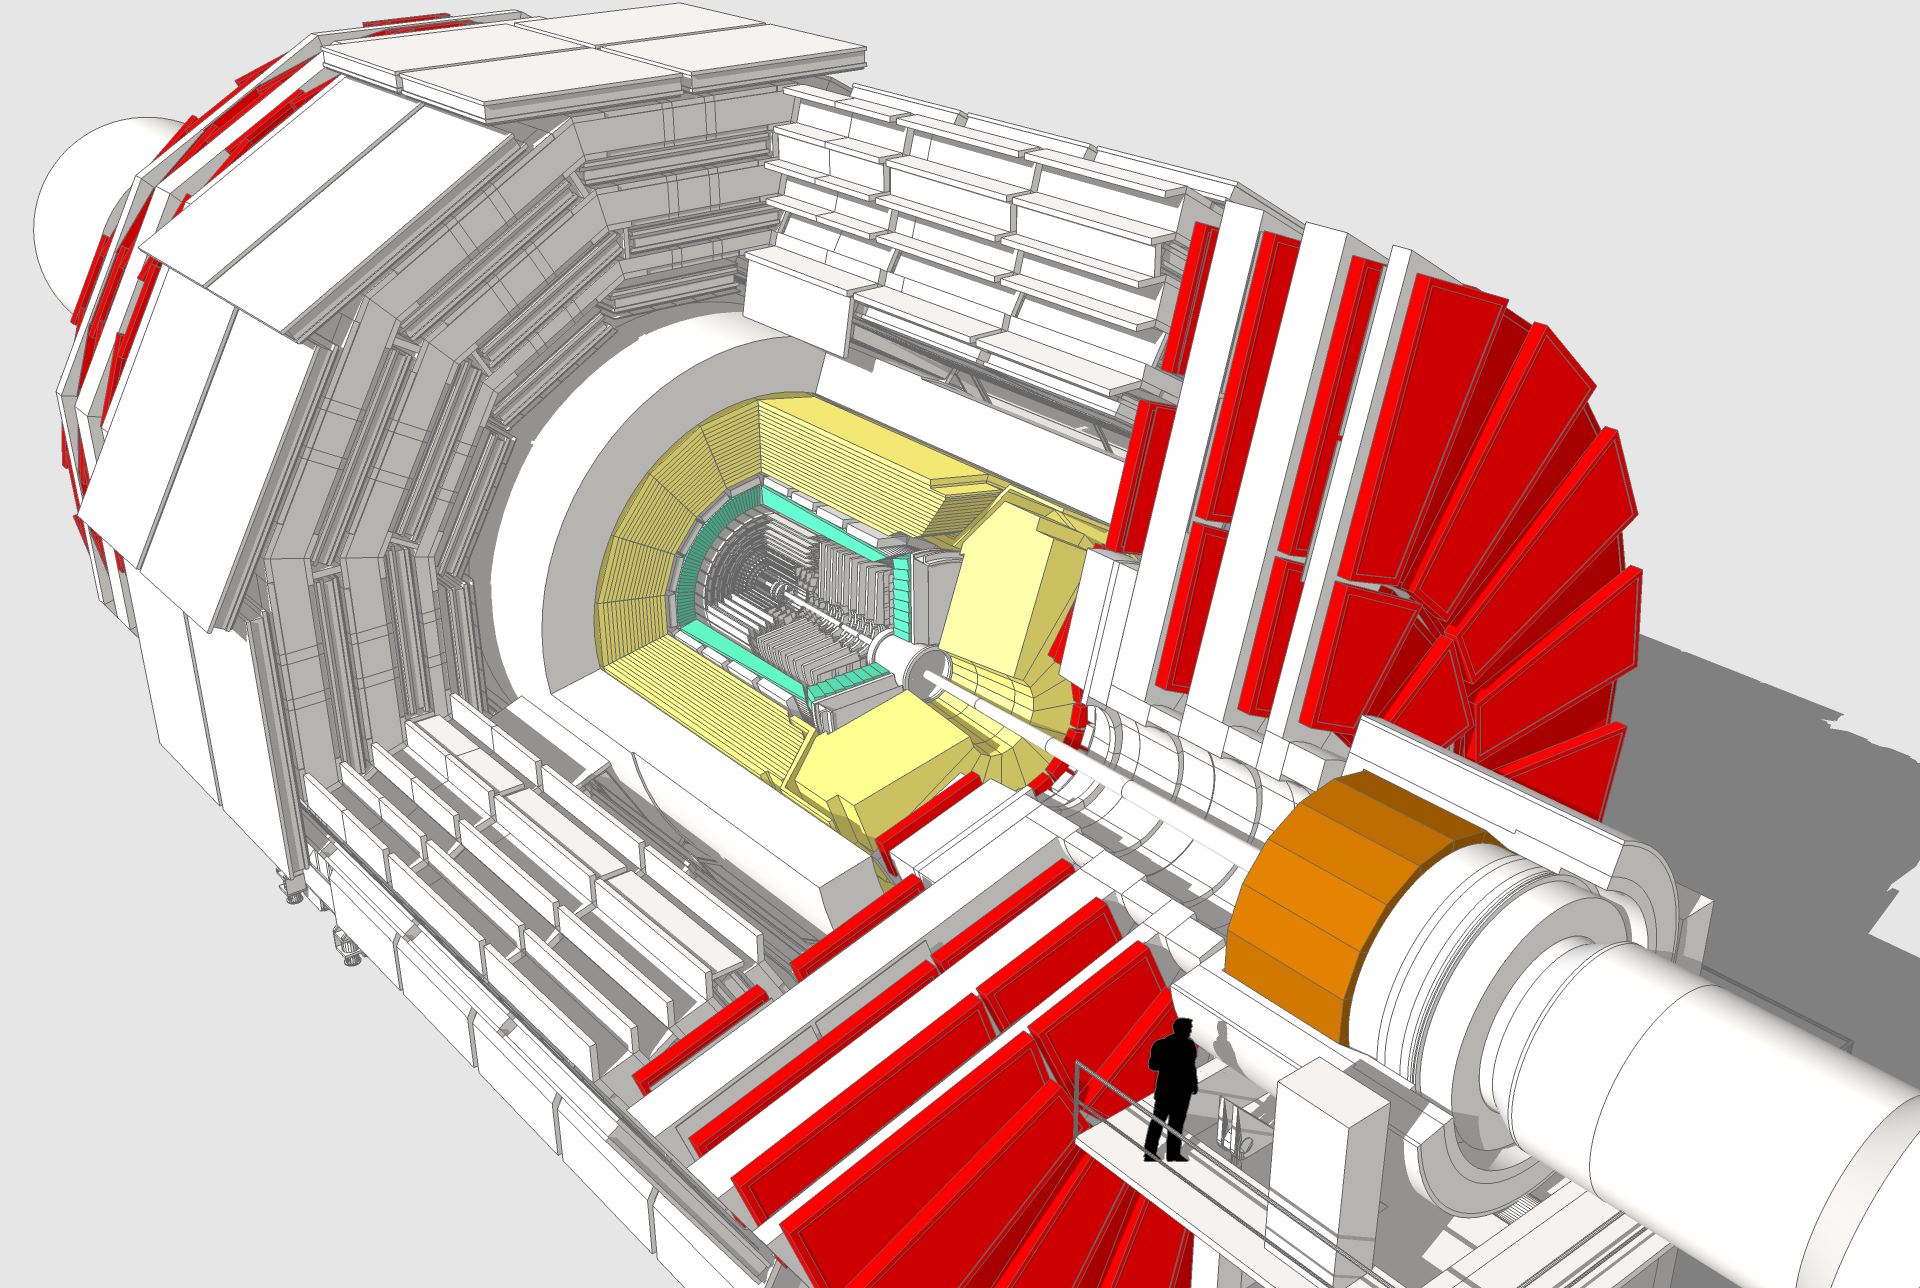
\includegraphics[width=1\textwidth]{figures/cmsDetectorBasic.png}
	\caption{Cut-away view of the entire CMS detector.  Closest to the proton-proton interaction point is the 
		silicon tracker, followed by the Electromagnetic Calorimeter, then the Hadronic Calorimeter, and the 
	magnet.  Outside the magnet solenoid are the muon detectors.}
	\label{fig:layersOfCMS}
\end{figure}


Surrounding the silicon tracker was the second of three sub-detector systems enclosed in the full strength magnetic field, the
lead-tungstate crystal (PbWO$_{4}$) Electromagnetic Calorimeter (ECAL).  The ECAL was an absorption calorimeter that
detected photons produced by pp interactions, and distinguished electrons and positrons from other charged 
particles detected by the tracker.  Electrons, positrons and photons interacted with lead-tungstate nuclei 
through bremsstrahlung and electron-positron pair production processes, and produced showers of lower energy
electrons and positrons.  Through Coulomb interactions, these lower energy particles excited atomic electrons
of lead-tungstate nuclei to higher energy, meta-stable bound states.  When these atomic electrons transitioned
back to the ground state, visible light photons were produced.  High energy photons, electrons and positrons 
produced by pp interactions were detected by measuring the visible light produced in lead-tungstate crystals.

Wrapped around the ECAL was the last of three sub-detector systems enclosed in the full strength magnetic field, the brass and 
plastic scintillator Hadronic Calorimeter (HCAL).  Built from alternating layers of brass absorber and scintillating
plastic tiles, the HCAL was a sampling calorimeter that detected charged and neutral hadrons.  Charged and 
neutral hadrons that travelled through the tracker and the ECAL interacted with bound nucleons in brass absorber layers
through diffractive and inelastic scattering processes.  Scattering events produced showers of lower energy hadrons, which
travel through nearby scintillating plastic tiles.  Interactions between low energy hadrons and molecules in
the plastic excited the molecules to meta-stable states.  When excited molecules transitioned back to the ground 
state, visible light photons were emitted.  High energy charged and neutral hadrons produced by pp interactions 
were detected by measuring the visible light produced in scintillating plastic tiles.

Outside the HCAL was the 3.8$\unit{T}$ magnet.  The magnetic field was generated by running a current of 
$\lesssim$18 thousand amps through superconducting wire wound into a solenoid.  The wire, made from a niobium alloy, was 
cooled to a superconducting state using a liquid helium adsorption refrigerator and liquid nitrogen precooling 
system.  The cryogenic system and magnet were supported by a separate structure built from iron, steel and titanium.  The
large volume of material linked to the magnet and support systems provided a barrier through which only muons 
could penetrate.

Surrounding the magnet was the fourth sub-detector system used to detect particles, the muon detectors, which resided 
in the magnet return yoke where the magnetic field strength was between 1 and 3$\unit{T}$.  Three 
different technologies - drift tubes (DT) in the lowest radiation regions, cathode strip chambers (CSC) in higher 
radiation regions, and resistive plate chambers (RPC) in all regions - were used to detect muons.  In detectors of all 
three technologies, muons travelled through pressurized gas chambers and ionized electrons from the gas along their 
trajectories.  Within the chambers, electric fields accelerated the ionized electrons towards conducting wires.  Muons 
were detected by measuring the charge collected by conducting wires.

Due to the enormous rate of pp collisions in which only elastic or diffractive scattering occurred, a two tiered trigger 
system was used to select events where energetic charged leptons, hadronic jets, photons, neutrinos or combinations 
thereof were detected.  The first tier of the trigger system processed information from the ECAL, the HCAL and the muon 
detectors in small regions where high energy particles were detected.  Regions in which the detected energy exceeded 
a preset threshold were then processed by the second tier of the trigger system.  In the second tier, reconstruction software 
was run in selected regions to identify charged leptons, photons, jets and neutrinos.  If a pp collision event produced one 
or more of these reconstructed particles that passed quality and energy cuts defined in the second tier, then all data 
from all four sub-detector systems for that event was read out and written to disk.

The accelerator which collided the proton beams, the coordinate system used to characterize the kinematics of detected 
particles, the silicon tracker, both calorimeters, the muon detectors and the trigger system are discussed in this chapter.

\section{The Large Hadron Collider}
\label{sec:lhcDescription}
Situated near Geneva, Switzerland and spanning the French-Swiss border, the CERN Large Hadron Collider (LHC) accelerated 
two counter-rotating proton beams in a 27 km circular tunnel (CITE) up to an energy of 6.5 TeV in 2015.  At several points along the tunnel 
the two beams collided, and surrounding one of these points the CMS experiment was built.

Several accelerator stages were used to create a proton beam in the LHC.  Summarized in Figure \ref{fig:accelComplex} \cite{DeMelis:2197559}, each 
proton beam began as isolated proton bunches ionized from hydrogen gas.  Proton bunches were first accelerated by a linear 
accelerator, LINAC 2, and were then injected into the circular Proton Synchrotron (PS) accelerator.  Protons were accelerated 
to an energy of 26 GeV by the PS, and then were injected into the circular Super Proton Synchrotron (SPS) accelerator.  
The SPS accelerated proton bunches to an energy of 450 GeV, which were subsequently injected into the LHC.  Once the SPS 
injected the desired number of proton bunches to fill two beams, the LHC accelerated both beams to the desired energy, 
and focused the beams to increase the rate of pp collisions.  In 2015 each beam was accelerated to an energy of 6.5 TeV, and 
contained as many as 2300 proton bunches, each separated by 25 \ns.

\begin{figure}[ht]
	\centering
	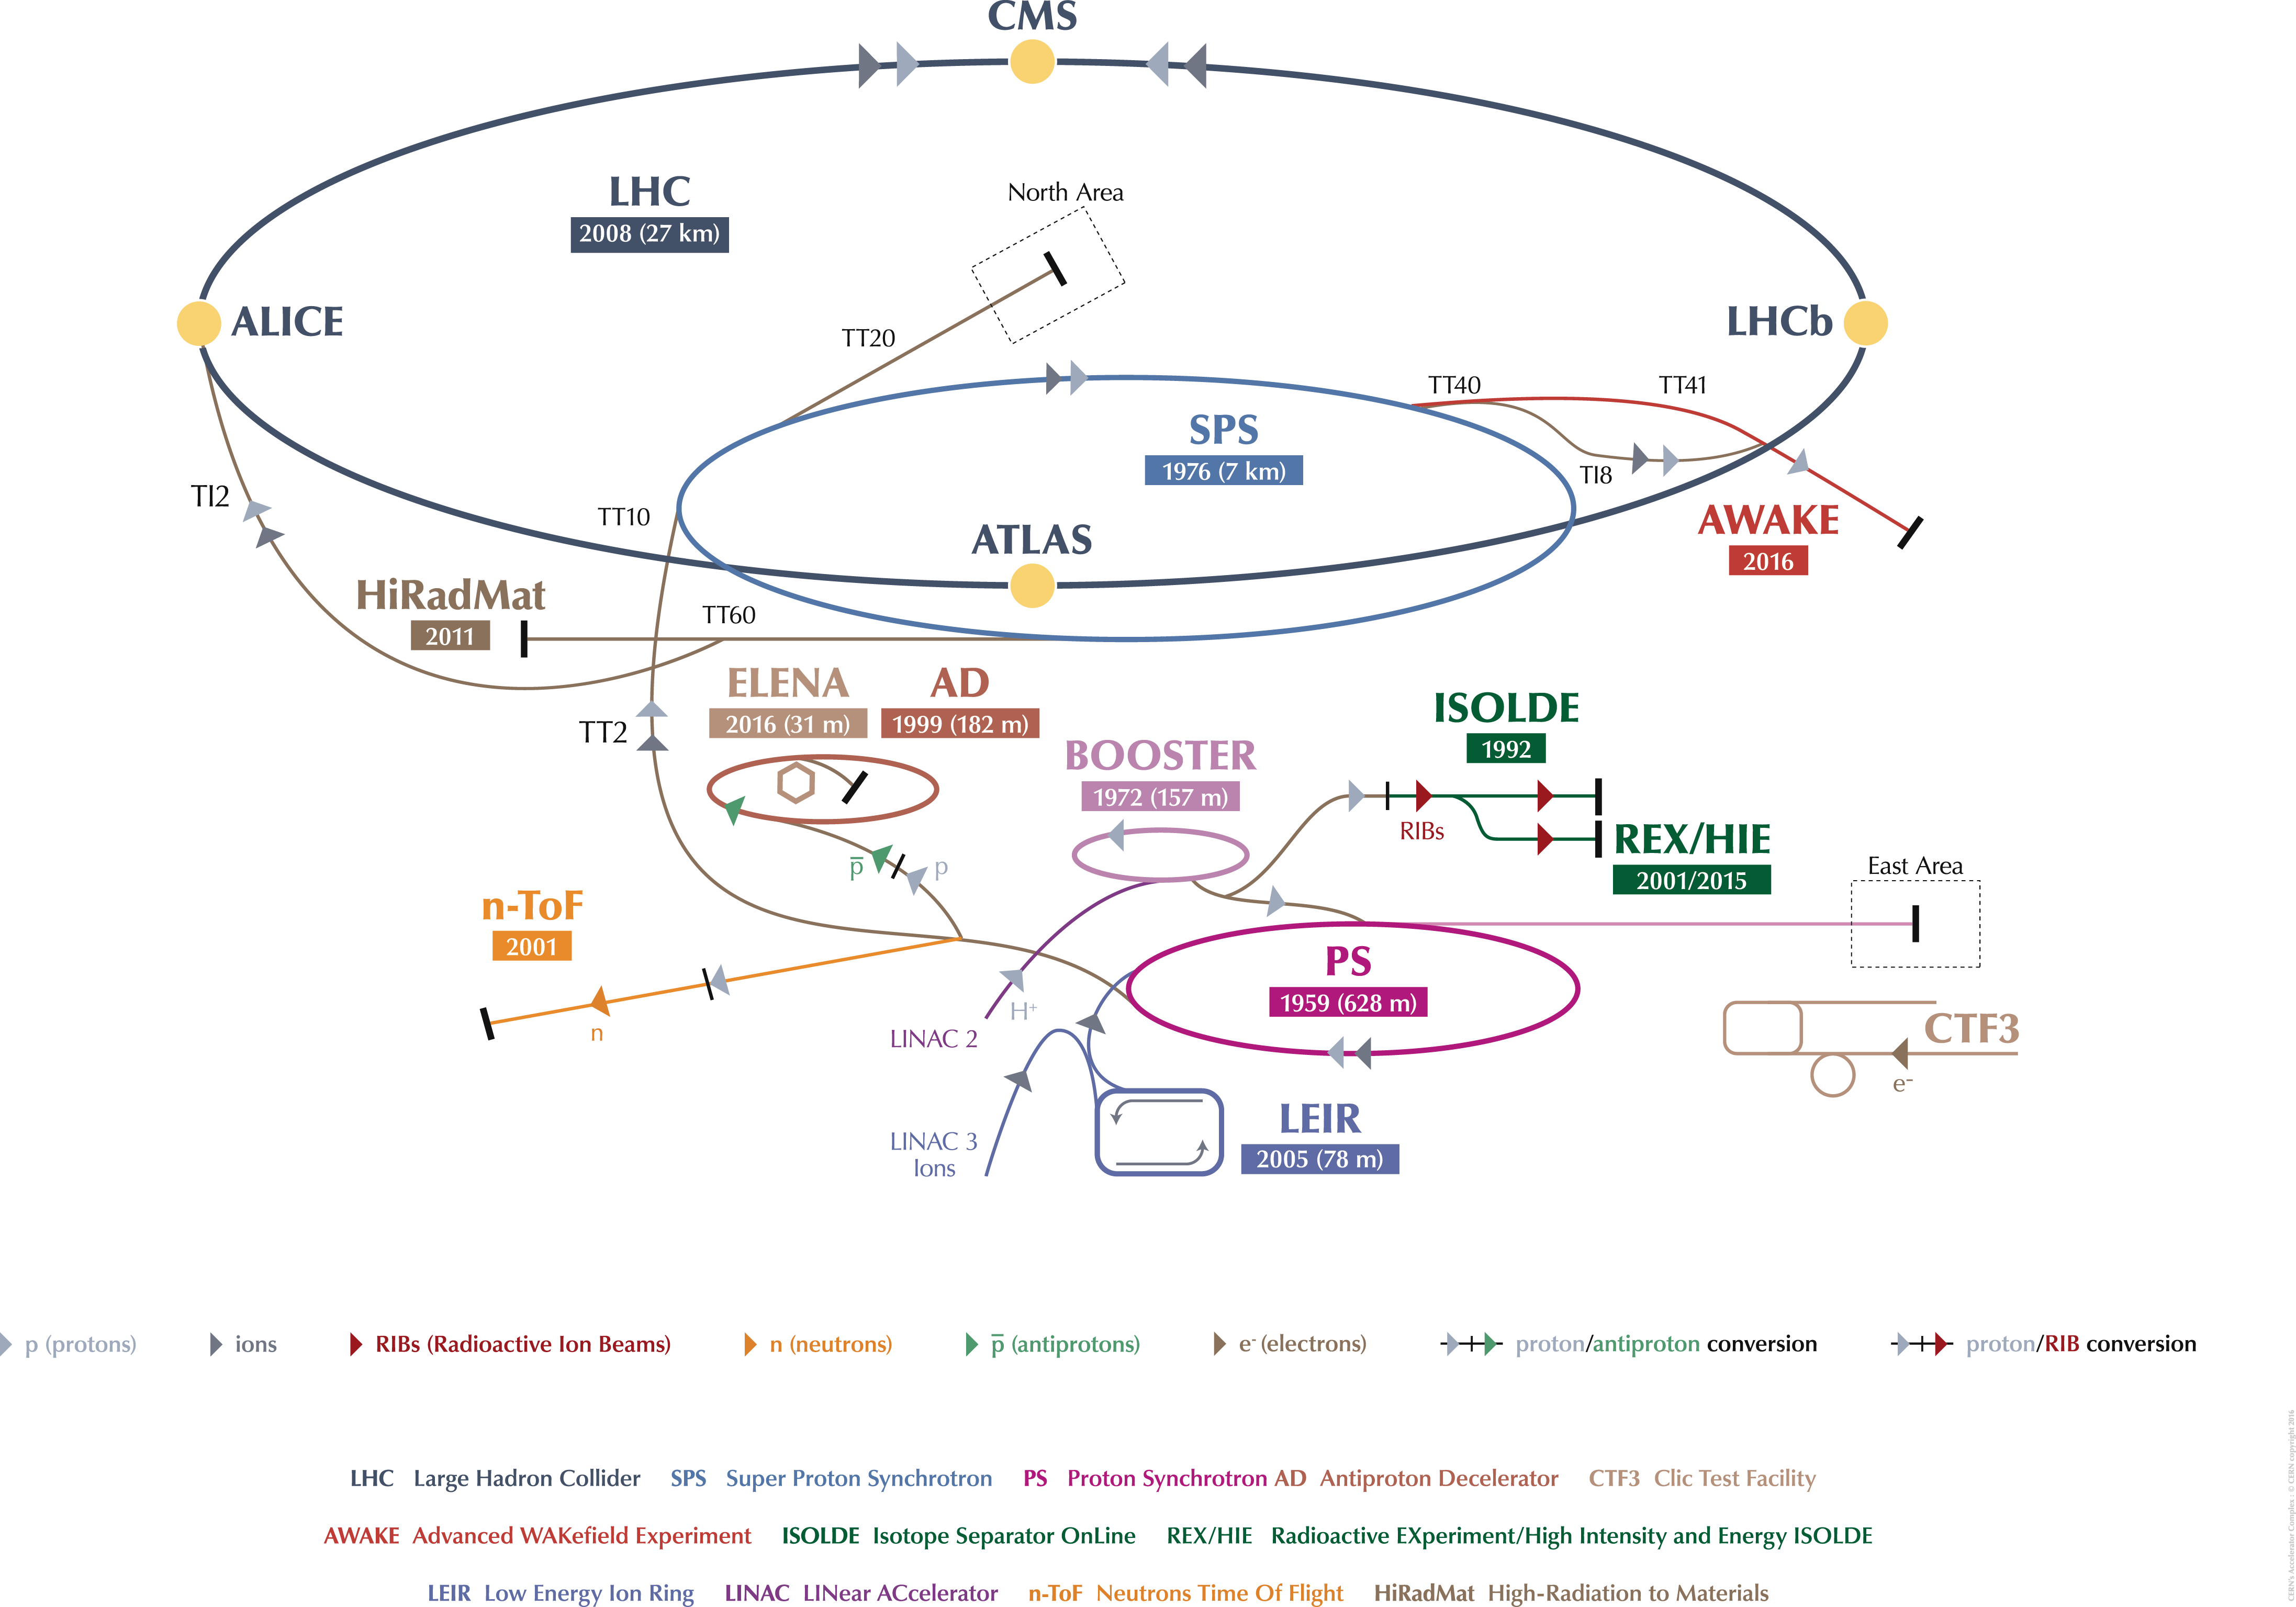
\includegraphics[width=1\textwidth]{figures/CERNAcceleratorComplex.png}
	\caption{The CERN accelerator complex.  Protons are ionized from hydrogen, then are accelerated to higher 
	energies by LINAC 2, the PS, and finally the SPS before entering the LHC.}
	\label{fig:accelComplex}
\end{figure}


In the LHC tunnel, superconducting radio-frequency (RF) cavities accelerated proton bunches, and magnets steered and 
focused the beams towards the collision point at the heart of CMS.  Sixteen RF cavities (8 per beam) accelerated proton 
bunches to an energy of 6.5 TeV, and also served as a control system in which protons in any bunch moving too quickly 
were slowed, while protons moving too slowly experienced greater acceleration.  Dipole, quadrupole and higher order 
magnets operated at magnetic field strengths up to 8$\unit{T}$ steered the beams around the LHC, and focused them 
on the nominal interaction point inside CMS to increase the rate of pp interactions.  Using these technologies, the  
LHC collided protons at rates approaching $6 \times 10^{33} \frac{protons}{cm^{2}s}$ during 2015 data taking.  
Spanning September through November 2015, 25 \ns collisions delivered by the LHC allowed CMS to record 2.6 $fb^{-1}$ 
of data at $\sqrt{s} =$ 13 TeV.

\section{The CMS Coordinate System and Kinematic Variables}
\label{sec:coordinateSystemAndKinematicVars}
A coordinate system and variables was used to characterize the kinematics of detected particles.  
The right-handed coordinate system was defined with the $z$ axis pointed in the direction 
of the counter-clockwise rotating beam, the $y$ axis pointed up towards the surface, and the $x$ axis pointed towards 
the center of the LHC ring, as shown in Figure \ref{fig:cmsAndCoordinateSystem}.  In this coordinate system particle 
trajectories were measured using two angular variables, $\phi$ and $\eta$, that were defined in terms of angles 
in two coordinate planes.  $\phi$ was defined as the angle in the $x-y$ plane, and took values between 0 and $2\pi$.  
The angle $\theta$ in the $y-z$ plane, which was 0 ($\frac{\pi}{2}$) when pointing along the $z$ ($y$) axis, was 
transformed into pseudorapidity $\eta$ through the following function:

\begin{equation}
	\eta \equiv -\ln{\tan{\frac{\theta}{2}}}
\end{equation}


\begin{figure}[ht]
	\centering
	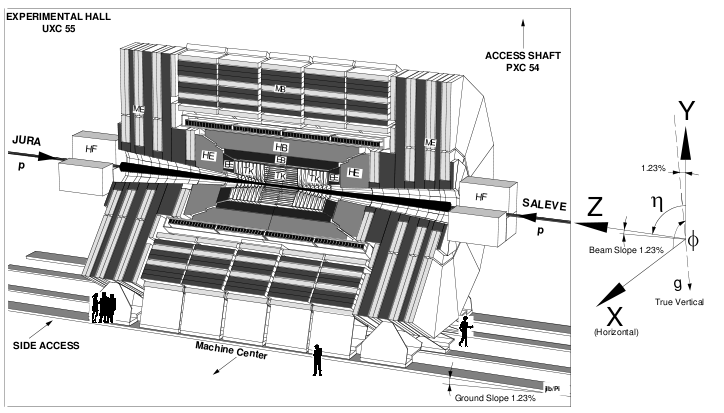
\includegraphics[width=1\textwidth]{figures/cmsDetectorAndCoordinateSystem.png}
	\caption{All CMS detector components and the coordinate system used to describe particle kinematics.}
	\label{fig:cmsAndCoordinateSystem}
\end{figure}


A pseudorapidity of 0 pointed along the $y$ axis, while a pseudorapidity of $\infty$ pointed along the $z$ axis.
An equivalent definition of pseudorapidity in terms of the particle energy E and longitudinal 
momentum $p_{z}$ in the massless particle limit was:

\begin{equation}
	\eta \equiv \frac{1}{2}\ln{\frac{E+p_{z}}{E-p_{z}}}
\end{equation}

Pseudorapidity was used to describe particle trajectories instead of the angle $\theta$ for several reasons.  Particles 
produced by pp interactions were often boosted along the $z$ axis, but the degree of boost was never well 
defined because the momenta of the interacting partons could never be measured.  This boost affected the 
trajectories of particles in $\theta$, but did not affect particle trajectories measured in $\eta$.  In 
addition, the particles that caused radiation damage in CMS sub-detector systems were produced at 
a rate that scaled linearly with $\eta$.  Thus, in discussions where radiation damage or particle 
isolation played a role, ideas could be more clearly articulated using $\eta$.

The main variables used to quantify the energy of a detected particle were transverse energy 
$E_{T} \equiv E/\cosh{\eta}$ and transverse momentum $p_{T} \equiv |p|/\cosh{\eta}$, while the distance between 
a particle and another point in the $(\eta, \phi)$ space was measured as $\Delta R \equiv \sqrt{\eta^{2} + \phi^{2}}$.  
Transverse momentum, the component of momentum perpendicular to the proton beam axis, and transverse energy, the 
analogous form of energy, were used because both were insensitive to the unknown momenta of the interacting partons.  
Explained in later chapters, the distance $\Delta R$ was measured between the trajectory of one particle 
and another point in the $(\eta, \phi)$ space.

\section{The Silicon Tracker}
\label{sec:siTrackerDescription}
Built from separate silicon pixel and silicon strip trackers, the silicon tracker detected charged particles  
and measured their momenta, and identified interaction vertices where charged particles were produced.  Closest 
to the beam axis was the pixel tracker, which used small silicon pixels to pinpoint pp interaction vertices 
with $\mu$m precision.  Surrounding the pixel tracker were larger silicon strip detectors that measured the 
momenta of charged particles.  Charged particles produced within the tracker acceptance of $|\eta| < 2.5$ ionized 
charge in the silicon pixel and strip trackers, and the measurement of this charge formed the basis for all tracker 
measurements.

The pixel tracker was built from small rectangular pixel detectors ($100 \times 150 \mu$m) organized in two 
structures based on $|\eta|$.  In the barrel region ($0 < |\eta| \lesssim 1.2$) where the rate of radiation damage was 
low, individual pixel detectors were arranged into three 53 \cm long concentric cylindrical shells centered on the 
$z$ axis, with radii of 4, 7 and 10 \cm relative to the $z$ axis.  The face of each barrel pixel pointed towards the interaction 
point, and, for reasons described later, their faces were aligned with the magnetic field direction.  In the endcap region 
($1.2 \lesssim |\eta| \leq 2.5$) where the rate of radiation damage was high, two layers of pixel detectors were 
installed in a turbine pattern as shown in Figure \ref{fig:pixelTracker} \cite{pixelCommissioning}.  These disks 
were placed at $|z| =$ 35 and 47 \cm away from the midpoint of the pixel barrel cylindrical shells, and covered 
radii between 6 and 15 \cm from the $z$ axis.  For reasons discussed later the face of each endcap region pixel 
pointed 20 degrees away from the interaction point.


\begin{figure}[ht]
	\centering
	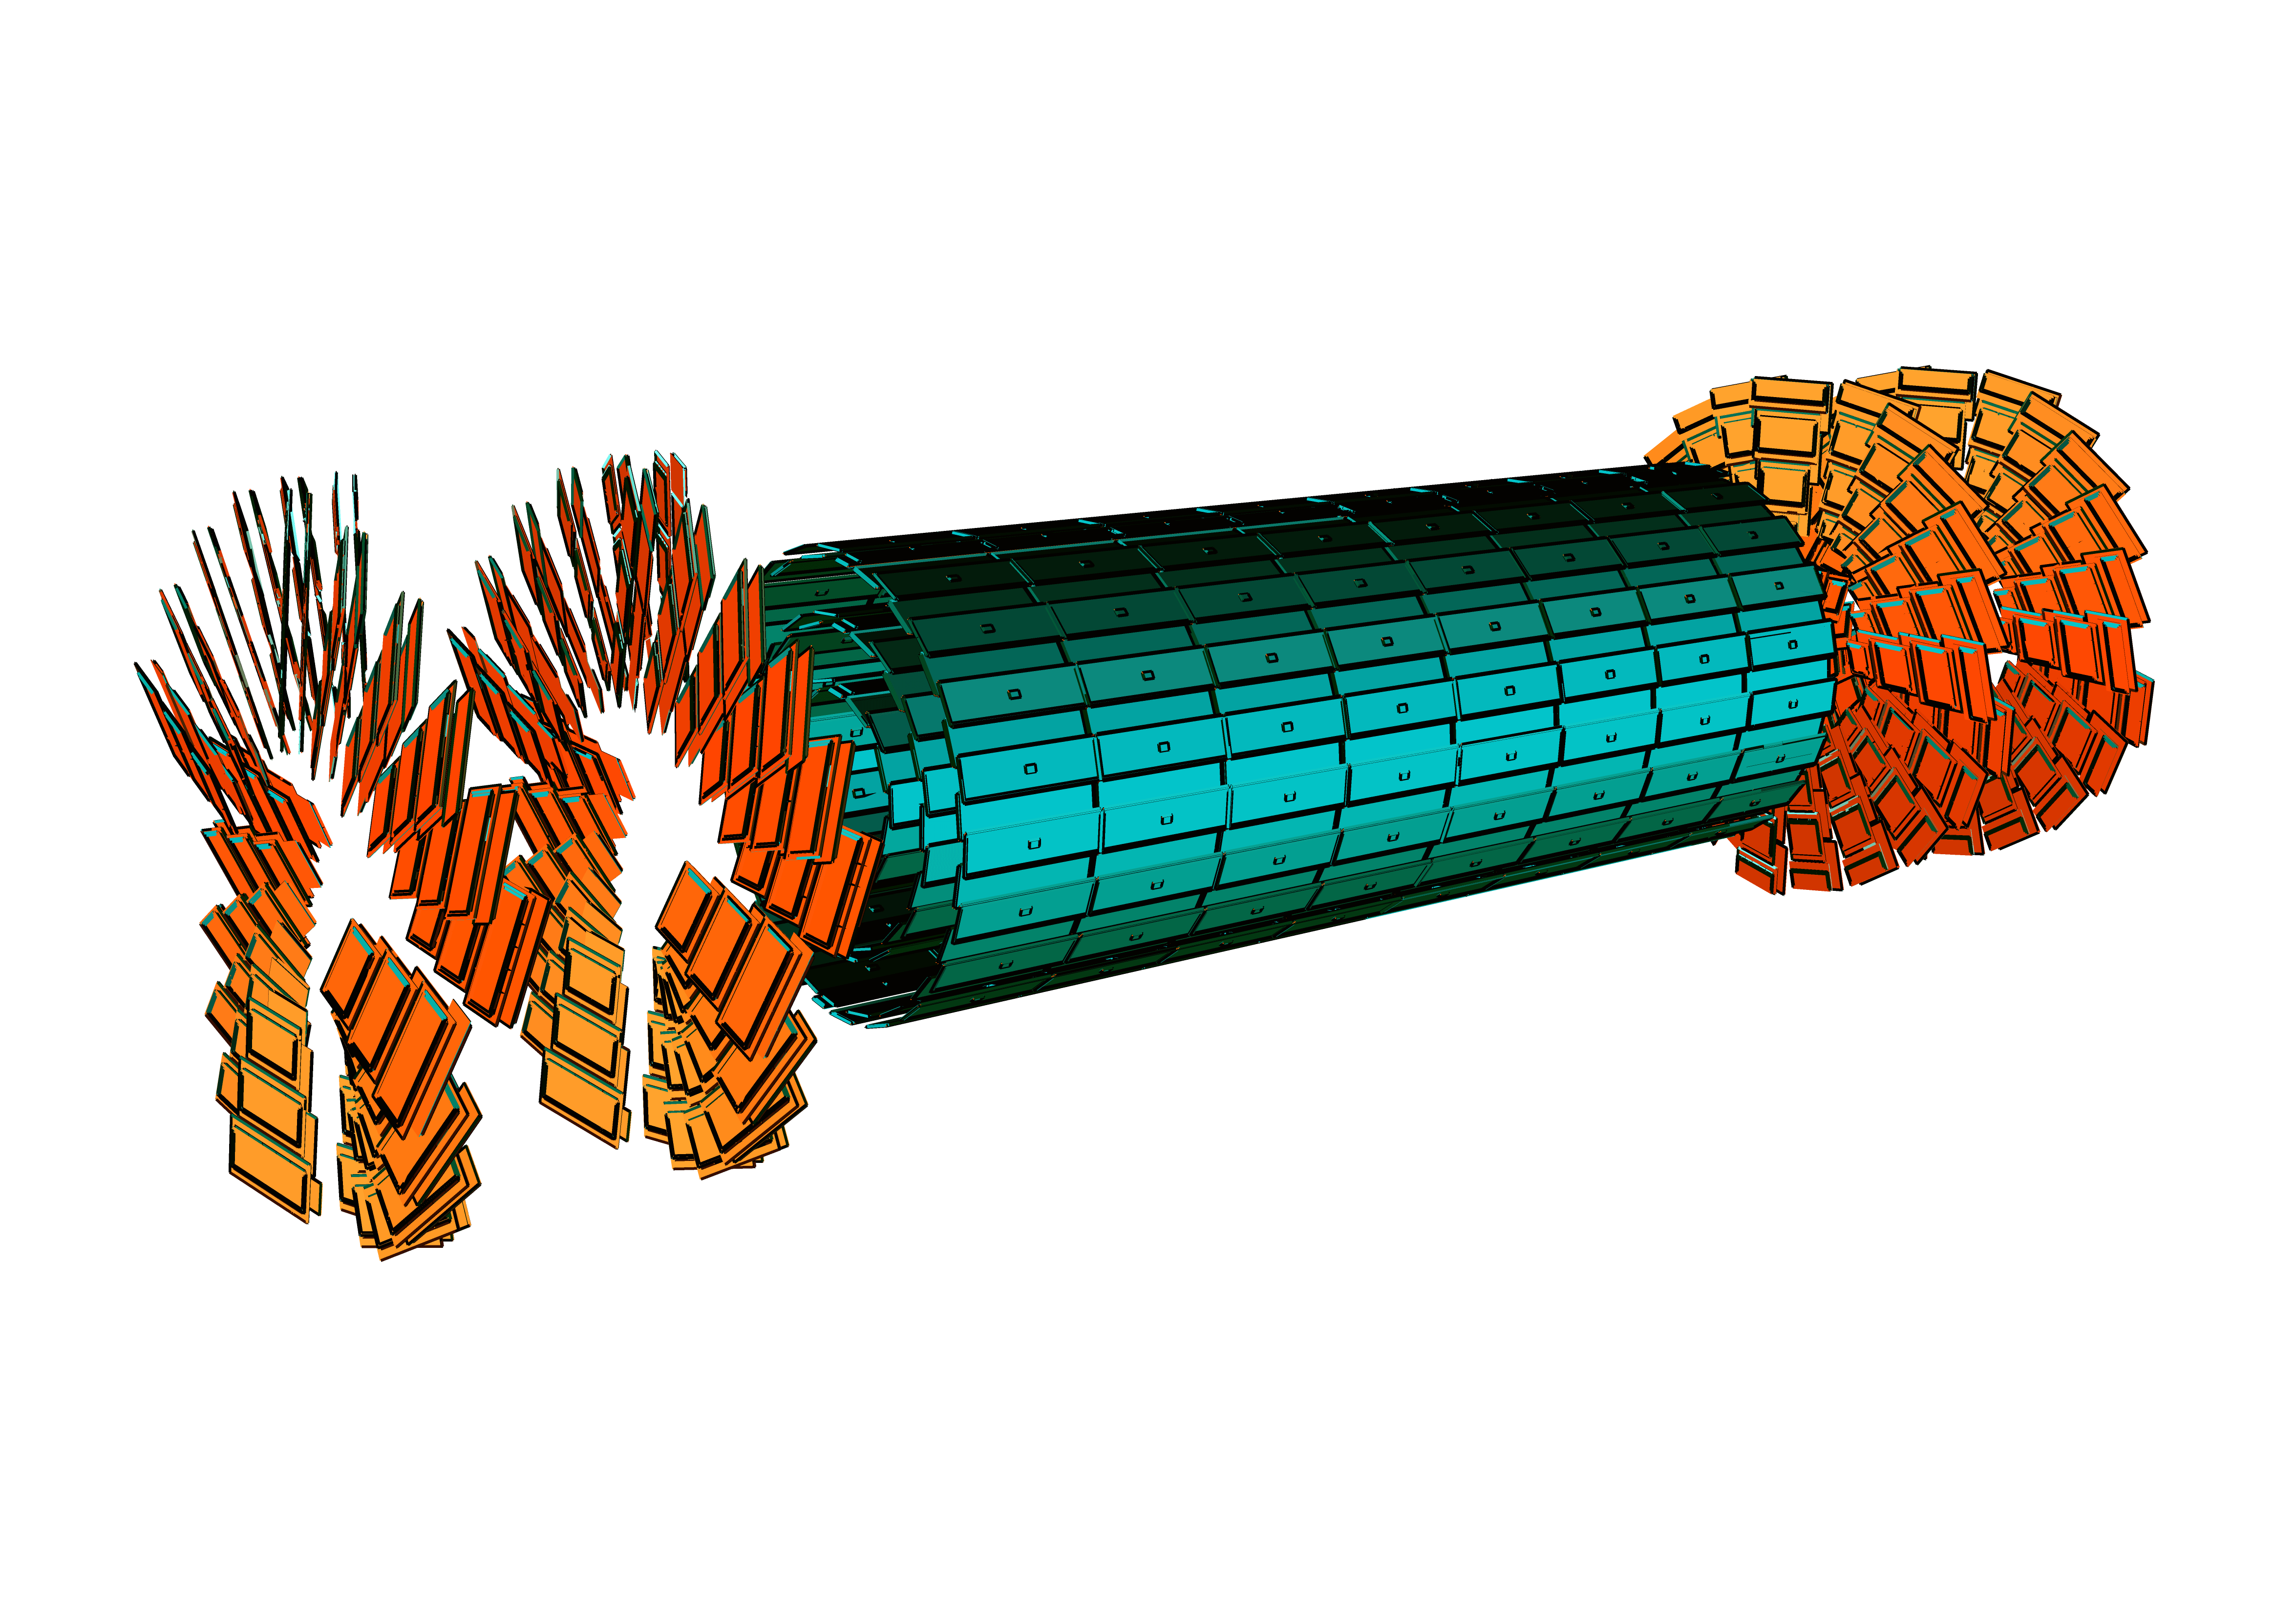
\includegraphics[width=0.8\textwidth]{figures/pixelDetectorSchematic.png}
	\caption{The barrel and endcap sections of the pixel tracker.}
	\label{fig:pixelTracker}
\end{figure}

Charged particles ionized charge in every pixel detector they hit, and this charge was measured by readout 
modules attached to groups of pixels\footnote{$\thicksim$16000 readout modules were connected to 66 million individual pixels}.  Each readout module created an 
electric field along the surface of several pixels that swept ionized charges into a charge collector.  The 
position resolution of pixel detectors improved when ionized charge from one charged particle was measured 
over a greater area, so all pixels were positioned relative to the magnetic field to create a 
Lorentz force that encouraged charges ionized in one pixel to migrate to nearby pixels.  The resulting pixel 
tracker configuration allowed interaction vertex coordinates to be measured with $\lesssim 20\mu$m resolution along the 
$z$ axis, and with $\lesssim 10\mu$m resolution in the plane perpendicular to the $z$ axis.

Located outside the pixel tracker, the silicon strip tracker was built from larger rectangular silicon detectors 
organized into four structures based on $|\eta|$, $|z|$ position and radius $r$ from the $z$ axis.  In the barrel region 
($0 < |\eta| \lesssim 1.2$), four cylindrical shells of 10 \cm $\times$ $80-120$ $\mu$m silicon strips were placed within 20 $< r <$ 55 \cm.  At
55 $< r < $110 \cm where radiation levels were much lower, six layers of thicker, larger surface area (25 \cm $\times$ $120-180$ $\mu$m) 
strips were placed in cylindrical shells for improved momentum resolution.  To improve track position resolution the two strip layers with smallest 
$|r|$ each contained two layers of silicon strips separated by a small distance and tilted relative 
to each other by 100 mrad.  For the same reason the first two of six strip detector layers in the region $r >$ 55 \cm 
were also built with the double layer design.  Similar to the pixel tracker, the strip tracker in the endcap region 
($1.2 \lesssim |\eta| \leq 2.5$) used strip detectors arranged in disks.  Three disk layers were installed between 
$1.2 \lesssim |\eta| \lesssim 2.3$, 20 $< r <$ 55 \cm and 65 $< |z| <$ 110 \cm, and nine disk layers with thicker strips were installed in 
the region $1.0 \lesssim |\eta| \lesssim 2.5$, 20 $< r <$ 110 \cm and 120 $< |z| < $ 280 \cm, as shown in Figure \ref{fig:stripTracker} \cite{cmsTDR}.  
To improve track position resolution two of the three inner disk layers, and three of the nine outer disk layers 
used two closely spaced silicon strips tilted by 100 mrad.  The faces of all strip detectors pointed at the interaction 
point.

\begin{figure}[ht]
	\centering
	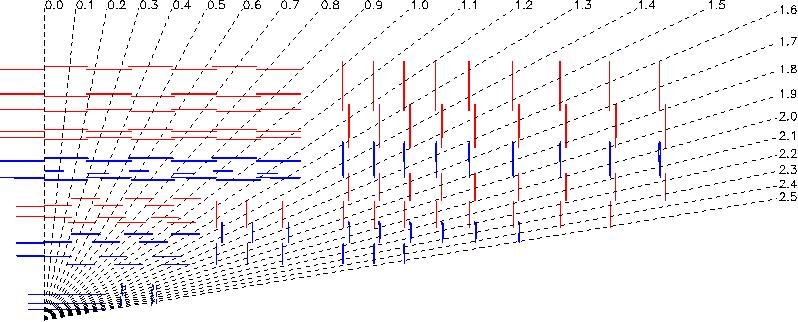
\includegraphics[width=0.8\textwidth]{figures/siliconStripAndPixelDetectorTwoDimView.png}
	\caption{The barrel and endcap sections of the silicon strip tracker for $\eta \geq 0.$ and one quadrant of $\phi$.  The pixel tracker is shown to scale in the bottom left corner.}
	\label{fig:stripTracker}
\end{figure}

Charged particles ionized charge in every strip detector they hit, and this charge was measured by readout 
modules attached to groups of strips\footnote{$\thicksim$15400 readout modules were connected to 9.6 million individual strips}.  Each readout module created an 
electric field along the surface of several strips that swept ionized charges into a charge collector.  The resulting 
strip tracker measured the $p_{T}$ of 100 GeV $p_{T}$ muons with resolution better than 2\% in the barrel, and 
better than 7\% in the endcap.

To measure the position and momenta of charged particles with the quoted resolutions, the alignment and calibration 
of the tracker were measured before and during pp collisions in 2015.  Before collisions, cosmic ray muons were 
used to measure the tracker alignment and momentum response, and derive calibration factors that accounted for 
changes in either.  During collisions $Z \rightarrow \mu\mu$ events and cosmic ray muon events were used to monitor 
and recalibrate the tracker alignment and momentum response.


\section{The Electromagnetic Calorimeter}
\label{sec:ecalDescription}

Surrounding the silicon tracker was the electromagnetic calorimeter (ECAL), which detected photons produced by 
pp interactions, and distinguished electrons and positrons ($e^{\pm}$) from other charged particles.  
The ECAL was an absorption calorimeter built from homogeneous, scintillating lead-tungstate (PbWO$_{4}$) crystals.  
In response to incident photons and $e^{\pm}$ with energy $\gtrsim$ 1 GeV, the ECAL crystals emitted 
amounts of visible light proportional to the incident particle energy.  The ECAL measured the energies of photons 
and $e^{\pm}$ with $0 < |\eta| < 3.0$ by measuring the amount of visible light produced by the lead-tungstate crystals.

The ECAL contained $\thicksim$76000 crystals divided into two $|\eta|$ regions based on the rate of radiation 
damage.  In the low $|\eta|$ barrel region ($0 < |\eta| < 1.479$) where the rate of radiation damage was low, 61200 
crystals of length 23 \cm (26 radiation lengths) were arranged in a cylindrical shell, and pointed near the 
interaction point.  The front face of each crystal measured $\thicksim$22 $\times$ 22 \mm, and resided 129 \cm 
from the beam axis, $\thicksim$19 \cm away from the outer most silicon tracker barrel layer.  In the high $|\eta|$ 
endcap region ($1.479 < |\eta| < 3.0$) where the rate of radiation damage was high, 14648 crystals (half in each 
endcap) of length 22 \cm (25 radiation lengths) were installed in a disk, and each crystal pointed near the interaction 
point.  The front face of endcap crystals measured $\thicksim$29 $\times$ 29 \mm, and sat behind two layers of 
thick lead absorber and thin silicon detectors that constituted the preshower detector.  The preshower 
mitigated radiation damage to endcap region lead-tungstate crystals, and improved the spatial resolution with 
which endcap region electromagnetic showers were studied.  A partial view of the ECAL barrel, endcap and 
preshower detectors is shown in Figure \ref{fig:ecalEBEEandES} \cite{ecalTDR}.

\begin{figure}[ht]
	\centering
	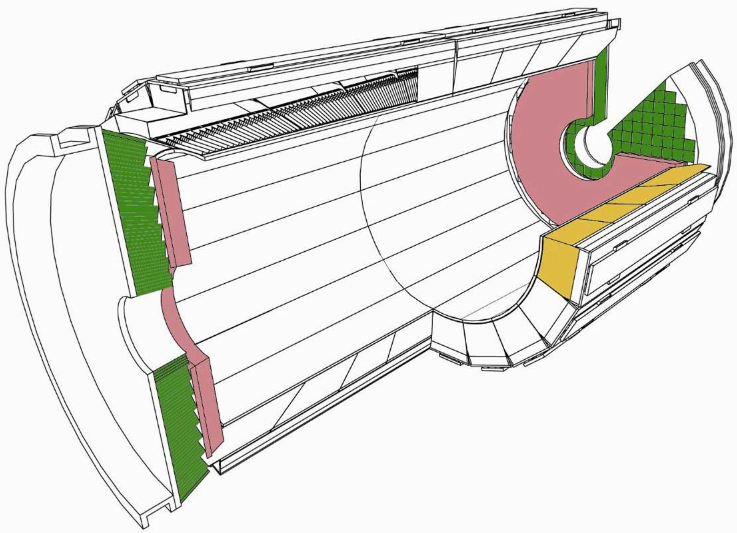
\includegraphics[width=0.8\textwidth]{figures/ecalBarrelEndcapAndPreshower.png}
	\caption{The ECAL barrel, endcap and preshower detectors.}
	\label{fig:ecalEBEEandES}
\end{figure}


Photons and $e^{\pm}$ that impinged on the ECAL interacted with lead-tungstate nuclei.  Incident $e^{\pm}$s interacted 
with lead-tungstate nuclei through the bremsstrahlung process and produced gamma rays.  Subsequently, gamma rays 
interacted with lead-tungstate nuclei and were converted into $e^{-}e^{+}$ pairs.  For every $e^{\pm}$ 
that impinged on the ECAL, the cycle of bremsstrahlung followed by pair conversion repeated many times, 
and a shower of lower energy $e^{-}$s and $e^{+}$s was made.  Every energetic photon that impinged on the 
ECAL first interacted with a lead-tungstate nucleus and converted into an $e^{-}e^{+}$ pair, then this pair underwent 
repeated cycles of bremsstrahlung followed by pair conversion, and a shower of lower energy $e^{-}$s and $e^{+}$s was made.  The crystal lengths 
guaranteed an average incident photon or $e^{\pm}$ lost more than $99.999$\% of its incident energy through 
radiative processes before leaving the ECAL, so the cycle of bremsstrahlung followed by pair conversion 
stopped when the incident particle energy was too low to produce gamma rays through bremsstrahlung.  The 
transverse size of each crystal was large enough that a 3 $\times$ 3 crystal grid contained the full shower 
created by an incident photon or $e^{\pm}$ that did not interact with the silicon tracker.

Showers of $e^{-}$s and $e^{+}$s interacted with lead-tungstate atoms and quickly produced distinguishable 
signals that determined the energies of incident photons and $e^{\pm}$s.  Coulomb interactions 
transferred several eV of energy from shower $e^{\pm}$s to atomic electrons bound to lead-tungstate nuclei.  
In addition, relativistic shower $e^{\pm}$s produced Cherenkov photons with several eV of energy, and 
these Cherenkov photons were absorbed by atomic electrons bound to lead-tungstate nuclei.  The atomic 
electrons were excited to meta-stable states, and in $\lesssim$ 20 \ns more than 80\% of atomic electrons 
returned to their ground states by emitting scintillation photons in the visible light regime.  The total energy of 
scintillation photons was proportional to the incident photon or $e^{\pm}$ energy, so the energies 
of scintillation photons were measured to determine the energy of the incident photon or $e^{\pm}$.  Scintillation  
photons were emitted in all directions, but needed to be directed towards the photodetectors at the back faces of the crystals.  To 
maximize the fraction of photons which reached the photodetectors, 5 faces of each crystal were polished 
to reduce the impact of surface impurities or imperfections, each crystal was wrapped in a reflective, 
non-absorbing material, and 17 different crystal shapes (all rectangular) were used to minimize gaps 
between crystals.  Scintillation photons from groups of 5 $\times$ 5 crystals were measured by avalanche 
photodiodes in the barrel region, and vacuum photo-triodes in the endcap region.  Both types of 
photodetectors converted scintillation photons into electric charge, and the amount of charge was measured 
to determine the energy of the incident photon or $e^{\pm}$.  With these technologies, the ECAL measured 
the energy of a 100 GeV photon or $e^{\pm}$ with resolution better than 1\%, and measured the energy of any 
incident photon or $e^{\pm}$ with resolution given by:

\begin{equation}
	\frac{\sigma_{E}}{E} = \frac{2.8\%}{\sqrt{E/(1 GeV)}} \oplus \frac{0.128 GeV}{E} \oplus 0.3\%
\end{equation}

To measure photon and $e^{\pm}$ energies with the quoted resolution, the ECAL was calibrated before 
and during 2015 pp collisions.  Before collisions, the ECAL was calibrated based on 2012 pp collision 
data.  Once collisions began, data collected from collision events was used by several methods 
to derive ECAL calibration constants for every lead-tungstate crystal.  The following quantities 
were measured for every crystal in millions of events:

\begin{itemize}
	\item $\pi^{0}/\eta$ masses through their decays to $\gamma\gamma$
	\item the average crystal energy in randomly selected events 
		(considering many randomly selected events, the energy measured should be symmetric in $\phi$.  Thus, within one $\phi$ ring each crystal should measure the same average energy)
	\item the ratio $\frac{E_{T,ECAL}}{p_{T,tracker}}$ for isolated electrons coming from W or Z boson decays
\end{itemize}

and relative calibration constants were derived such that every crystal had the same calibrated response.  
Then, the absolute scale of each crystal's response was calibrated using $e^{\pm}$ from 
$Z \rightarrow e^{\pm}e^{\mp}$ decays.  In events where a Z boson decayed to an $e^{\pm}e^{\mp}$ pair, the 
crystal responses were corrected so that the average mass of all $e^{\pm}e^{\mp}$ pairs was equal to 
the true Z boson mass.

\section{The Hadronic Calorimeter}
\label{sec:hcalDescription}
Surrounding the ECAL was the hadronic calorimeter (HCAL), which detected charged and neutral hadrons.  The 
HCAL was a sampling calorimeter built from alternating layers of thin scintillating plastic tiles and thick 
metal absorber plates.  Hadrons impinging on the HCAL with energy $\gtrsim$ 1 GeV interacted with the metal absorbers and produced amounts 
of visible light in the scintillating tiles proportional to their incident energies.  The HCAL 
measured the energies of hadrons with $0 < |\eta| < 3.0$ by measuring the amount of visible light produced 
by the scintillating tiles.

The HCAL consisted of 17 scintillating tile layers separated by 17 metal absorber layers.  Similar to the ECAL, the 
HCAL was divided into two $|\eta|$ regions based on the rate of radiation damage.  In the low $|\eta|$ barrel 
region ($0 < |\eta| < 1.4$), scintillating tiles and metal plates were organized into 2304 towers, and each 
covered a $\Delta\eta \times \Delta\phi$ area of $0.087 \times 0.087$ to match the area covered by a 5 $\times$ 5 grid of 
ECAL crystals in the barrel region.  In every tower the first and last metal absorber layers 
were made from 5 \cm thick steel to support the $\thicksim$1130 tons resting on the HCAL barrel.   All other layers 
were made from brass of the same thickness to minimize costs.  To increase the visible light produced by particles 
leaving the ECAL, the first layer of scintillating tile was 9 \mm thick , and tiles 
used in subsequent layers were 3.7 \mm thick.  The towers were arranged in a cylindrical shell, and each tower 
pointed towards the interaction point.  In the high $|\eta|$ ($1.3 < |\eta| < 3.0$) endcap region, scintillating 
tiles and absorber plates were assembled into 2304 towers (1152 per endcap) with variable widths in $\Delta\eta$ and 
$\Delta\phi$.  Towers that covered $1.3 < |\eta| \leq 1.74$ used absorber plates and scintillating tiles with 
the same thickness and $\Delta\eta \times \Delta\phi$ area as those in the barrel region.  At higher $|\eta|$, absorber 
plates and scintillating tiles with the same thickness and larger $\Delta\eta \times \Delta\phi$ area were used 
such that each tower covered the same area as a 5 $\times$ 5 grid of ECAL endcap crystals.

Hadrons that impinged on the HCAL interacted with nuclei in metal absorber layers.  Diffractive and fully 
inelastic collisions between incident hadrons and absorber nuclei produced showers of lower 
energy hadrons that traveled into the nearest scintillating tile layers.  The amount of metal absorber 
(5.15 to $\thicksim$9 interaction lengths) guaranteed that every hadron that impinged on the HCAL experienced, 
on average, at least 5 fully inelastic collisions, and at least 5 diffractive collisions.  Incident hadrons 
with higher energy produced showers with greater numbers of lower energy hadrons.  Upon entering a plastic tile, 
low energy charged hadrons in a shower transferred several eV of energy to plastic molecules through Cherenkov radiation 
and Coulomb interactions.  Each energy transfer excited a plastic molecule into a higher energy, meta-stable 
molecular state.  These molecules usually de-excited through the Forster transfer, in which energy was 
transferred to nearby scintillator molecules without the emission of radiation.  Mixed throughout every 
plastic tile was a cerium based scintillator, whose molecules were excited to higher energy molecular 
states through Forster transfer.  In $\thicksim$5 \ns, the cerium based scintillator molecules de-excited by emitting 
visible light in every direction.  To detect this scintillation light, an optical fiber was 
embedded near the perimeter of every tile in the shape of the sigma ($\sigma$) character.  The tiles were wrapped in 
a reflective, non-absorbing material to maximize the amount of scintillation light which reached the optical 
fibers.  Upon reaching the surface of a fiber, scintillation light was absorbed and re-emitted at 
a longer wavelength in the core of the fiber, along the fiber axis.  Longer wavelength light was used to reduce 
transmission losses encountered when transmitting the light to a photodetector.  The light produced in all 17 scintillating 
layers of a tower is sent to the same photodetector (hybrid photodiodes were used in the HCAL barrel and endcap), and 
the photodetector converted the light into electric charge.  Charge was measured from every tower to determine 
the energy of hadrons which impinged on the HCAL.  After calibrations the HCAL measured the energy of hadrons
with the following resolution:

\begin{equation}
	\frac{\sigma_{E}}{E} = \frac{84.7\%}{\sqrt{E/(1 GeV)}} \oplus 7.4\%
\end{equation}

To maintain the energy resolution of the HCAL, the amount of light measured from towers of scintillating tiles 
was monitored and calibrated before and during 2015 collisions.  Before collisions, a radioactive source 
with known radioactivity was lowered into the HCAL, and the amount of scintillation light produced by each tile 
in response to the source was used to derive calibration constants.  Once collisions began, a laser system 
was used to monitor the decrease in transparency of optical fibers that transmitted scintillation light 
from plastic tiles to photodetectors.  From laser transparency data, relative calibration constants were 
derived that normalized the response of all towers to hadronic activity to the same value.  The absolute 
calibration was determined by selecting events in which a jet recoiled off a photon, or a Z boson that 
decayed to a $e^{\pm}e^{\mp}$ or $\mu^{\pm}\mu^{\mp}$ pair.  In such events, the absolute hadronic energy 
scale was calibrated relative to the electromagnetic energy scale derived from $Z \rightarrow e^{\pm}e^{\mp}$ 
events.  Furthermore, the precision of the absolute hadronic energy scale calibration was improved using 
dijet resonances like $W/Z \rightarrow jj$.

\section{The Muon Detectors}
\label{sec:muonDetectorsDescription}
Outside the magnet were gas ionization chambers used to detect muons.  Muons that traversed the chambers 
ionized charge along their trajectories, and the ionized charges drifted through the gas to anodes and 
cathodes.  The muon detectors measured the momenta of muons with $0 < |\eta| < 2.4$ by measuring the amount of 
charge collected on the anodes and cathodes.

Like the calorimeters, the muon detectors were separated into barrel and endcap sections.  Shown in Figure \ref{fig:muonBarrelAndEndcapDetectors}, in the barrel 
region ($0 < |\eta| < 1.2$) where the magnetic field strength, muon rate and neutron induced background 
rate were low, drift tubes (DTs) and resistive plate chambers (RPCs) were used to measure the positions and 
and momenta of muons, and the collision event that produced them.  In the endcap region ($1.2 < |\eta| < 2.4$) where 
particle fluxes and magnetic field strengths were higher, RPCs and cathode strip chambers (CSCs) were used 
to measure the quantities stated previously.

\begin{figure}[ht]
	\centering
	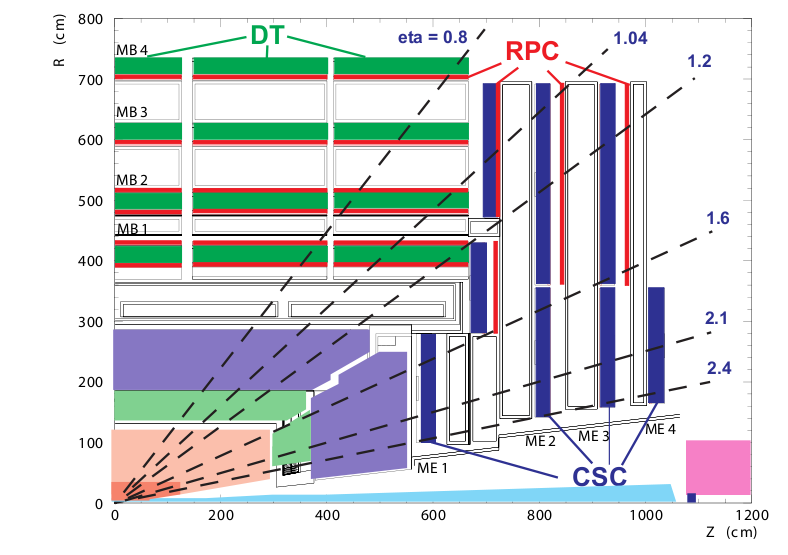
\includegraphics[width=0.8\textwidth]{figures/muonDetectorLayout.png}
	\caption{The barrel and endcap sections of the muon detectors for $\eta \geq 0.$ and one quadrant of $\phi$.  Shown 
		between the muon detectors and the interaction point are the magnet solenoid and return yoke, the HCAL, the ECAL, 
		and the silicon tracker.}
	\label{fig:muonBarrelAndEndcapDetectors}
\end{figure}


The DTs were organized into 5 wheels, each with 4 radial layers or 'stations', and 12 
$\phi$ segments per station covering 30 degrees in $\phi$.  Chambers in different stations were staggered 
so that high $p_{T}$ muons produced near the $\phi$ sector boundary hit at least three of four stations.  
DT chambers in the first, second and third stations each contained 12 planes of aluminum drift tubes - 8 
planes measured muons in r-$\phi$ coordinates, and 4 planes measured muons along the $z$ axis.  DT chambers 
in the fourth station were the same, but did not have the 4 planes for measurements in $z$.  In all DTs, ionized 
charge drifted 2 \cm or less to the nearest cathode or anode, and this allowed each station to measure muon 
vectors with resolution better than 100 $\mu$m in position, and $\thicksim$1 \mrad in $\phi$.  The large 
distance between the DTs and the interaction point meant that muons produced near the interaction point 
took 13 \ns or longer to reach the first DT station in any of the 5 wheels.  To identify the collision event 
that produced a muon, each DT chamber was paired with one or two RPCs that detected muons with $\thicksim$1 \ns 
resolution.  DT chambers in the first two stations were sandwiched between two RPCs, while each DT chamber 
in the third and fourth stations sat immediately behind one RPC relative to the interaction point.

Muons in the endcap region were detected by CSCs divided amongst four disks that faced the barrel region.  
The first disk, closest to the barrel DTs, was segmented into four radial layers (four rings of different  
radii).  As shown in Figure \ref{fig:muonBarrelAndEndcapDetectors}, the second and third disks were divided 
into two radial layers, and the fourth disk contained only one ring of CSCs.  The inner most radial layer in 
the second through fourth disks contained 18 CSCs, and all other radial layers contained 36 chambers.  Each 
CSC contained 6 gas gaps that were separated by 6 pairs of planes - one plane of cathode strips pointing in 
the radial direction, and one plane of anode wires that ran nearly perpendicular to the plane of cathode 
strips.  When a muon traversed a CSC, in a few \ns charge accumulated on the anode wires and was subsequently 
used for triggering.  Over a longer time period, charge collected on the cathode strips, and the position and 
trajectory of a muon was determined by measuring the shape of the charge distribution on the strips.  The 
cathode strips allowed muon vectors to be measured with resolution better than 200 $\mu$m in position, and 
$\thicksim$10 \mrad in $\phi$.  Similar to the barrel region DTs, the large distance between the interaction 
point and endcap CSCs meant that muons produced near the interaction point with $1.2 < |\eta| < 1.6$ took 
13 \ns or longer to reach the first CSC disk closest to the interaction point.  To identify the collision 
event that produced a muon, each CSC with $1.2 < |\eta| < 1.6$ sat in front of one RPC that detected 
muons with $\thicksim$1 \ns resolution.  For muons produced with $|\eta| > 1.6$, the distance between the 
interaction point and the first CSC disk was small enough that anode timing information from this disk 
unambiguously determined the collision event that produced a muon.

The muon detectors complimented measurements made by the tracker, and improved the resolution of muon 
momentum measurements for high $p_{T}$ muons relative to tracker only performance.  The 
strength of the magnetic field allowed the tracker to measure muon momenta in the $0 < |\eta| < 0.2$, $p_{T} <$ 
200 GeV phase space with 3 or more times better resolution than the muon detectors.  For higher $|\eta|$, this 
phase space extended to higher $p_{T}$.  As muon $p_{T}$s increased outside the tracker dominated phase 
space, muon trajectories approached straight line paths that degraded the tracker momentum resolution.  
Although the momentum resolution of the stand-alone muon detectors also degraded with increasing muon $p_{T}$, 
there is a significant advantage in combining muon and tracker measurements for high $p_{T}$ muons.  Muons 
that traversed the muon detectors traveled the same distance ($\thicksim$3 meters) or further that 
separated the interaction point from the magnet solenoid, but in a magnetic field opposite in direction.  
While travelling through several meters of muon detectors, even muons with $p_{T} = $ 1 TeV curved by tens 
of \cm.  By precisely measuring this curvature, combining muon detector and tracker information for a 
muon with $p_{T} =$ 1 TeV and $0 < |\eta| < 0.2$ improved the muon momentum resolution by $\thicksim$200\% relative 
to the momentum measurement made with the tracker alone.


\section{The Trigger System}
\label{sec:triggerDescription}
In 2015 the rate of pp collision events delivered by the LHC was several orders of magnitude greater than the 
rate that CMS could save collision events to permanent storage.  At that time the LHC collided two proton bunches 
at a rate of 40 MHz, and in nearly every collision $\gtrsim$1 GeV of energy was detected in CMS.  Due to the large cross 
section of QCD multijet processes and leptonically decaying heavy quark processes shown in Figure \ref{fig:smProductionXsxns}, CMS 
detected $\thicksim10^{6}$ collision events per second with energetic charged leptons or hadronic jets.  In 2015 
CMS could only write $\thicksim10^{3}$ collision events per second to permanent storage, so a two level trigger 
system was used during collisions ('online') to select the best events for physics analyses and detector calibration.

\begin{figure}[h]
	\centering
	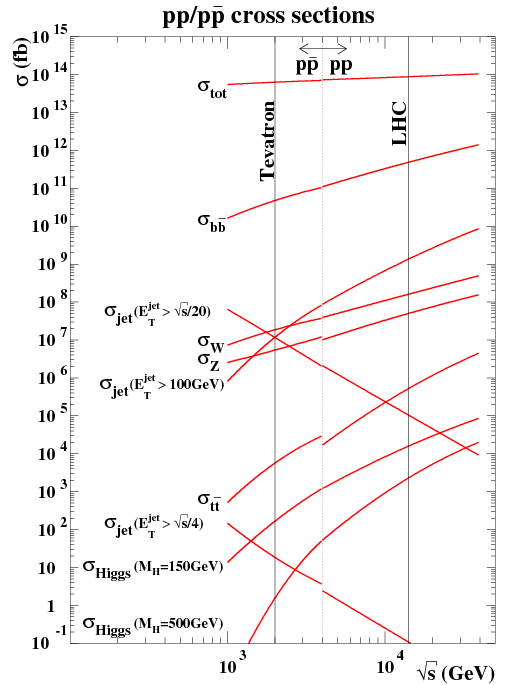
\includegraphics[width=0.6\textwidth]{figures/lhc_and_tevatron_cross_sections_2006.png}
	\caption{Production cross sections at the LHC and Tevatron as a function of center of mass energy.  Divide the cross section by $10^{5}$ to calculate 
	the approximate 2015 LHC production rate in events per second.}
	\label{fig:smProductionXsxns}
\end{figure}

By discarding collision events where no photons, charged leptons, hadronic jets, or neutrinos were 
detected, the Level-1 (L1) trigger system reduced the rate of collision events sent to the second 
level trigger system from 40 MHz to $\lesssim$ 80 kHz.  After every collision event, data from 
charge collection devices on the ECAL, the HCAL and the muon detectors was used to build 'trigger 
primitive' objects that represented photons, muons and other objects.  In $\thicksim$1 $\mu$s these objects, 
distinguished by $E_{T}$ values and $(\eta, \phi)$ coordinates, were built and sent to the L1 logic system located 
$\thicksim$20 meters from CMS.  Implemented in Field Programmable Gate Arrays, Application Specific 
Integrated Circuits and other custom and semi-custom hardware, the L1 logic system executed 
$\thicksim$200 algorithms in less than 1 $\mu$s that selected trigger primitive objects passing $E_{T}$ 
and $|\eta|$ selections.  The selection results were sent back to the detector, and the regions with one 
or more trigger primitive objects passing selections were processed by the second level trigger.

By selecting only the events needed for physics analyses and detector calibration, the second 
level, or High Level, trigger (HLT) reduced the rate of collision events written to permanent storage 
from $\lesssim$ 80 kHz to $\lesssim$ 1000 Hz.  First, all data from the tracker, both calorimeters and the muon 
detectors were transferred to commercial, multi-core processors where the HLT was run\footnote{the same HLT software was run on every processor}.  
Then, the HLT began by running a fast, simplified version of the full offline particle reconstruction software in small 
regions where L1 trigger algorithms were passed.  Then, $\thicksim$400 HLT algorithms running in 
parallel applied selection cuts ($E_{T}$, $|\eta|$, $\frac{E_{HCAL}}{E_{ECAL}}$, etc) to locally reconstructed particles in search of 
energetic photons, charged leptons, hadronic jets, and neutrinos.  If the event passed at least one 
HLT algorithm, then the data from the entire detector was written to permanent storage, and the event 
was assigned to one or more primary datasets based on the number of reconstructed particles required 
by the trigger\footnote{for example, an event that passed a trigger that required one muon was assigned to the SingleMuon primary dataset.}.
Considering events selected by all HLT algorithms, during 2015 pp collisions the rate of data written to 
permanent storage was $\lesssim 0.5$ gigabytes per second.


%Operations
%separation decreased to 25 ns to increase the instantaneous luminosity, and proton proton collisions continued until November.  From August until November, instantaneous 
%luminosities reached $5x10^{33} \frac{1}{cm^{2}s}$, but problems with the CMS
%magnet cooling system limited the amount of data collected to 2.6 $fb^{-1}$.  Decreasing the bunch spacing increased the sensitivity of every new physics search, but
%came with the cost of more proton proton interactions in every bunch collision, or pileup.  At 13 TeV the total inelastic cross section is approximately 70 mb \cite{Haevermaet}, 
%so for instantaneous luminosities between $3-5x10^{33} \frac{1}{cm^{2}s}$ in 25 ns running the expected pileup per bunch crossing is $8-13$, which is consistent with
%the pileup observed in 25 ns collision data.  Pileup increases the complexity of events$\footnote{15 inelastic pp collisions yield a total flux of particles similar to one top antitop quark pair event}$, and makes event reconstruction and offline analysis more challenging.


%\subsection{Compact Muon Solenoid Detector Overview}
%\begin{itemize}
%	\item trigger description, followed by particle flow event reconstruction
%\end{itemize}
%The Compact Muon Solenoid (CMS) experiment is designed to search for signs of new physics at the high energy and luminosity regime probed by the LHC.  The LHC was built
%as a discovery machine, so particular attention has been paid to searches for physics beyond the SM (BSM), such as supersymmetry and extensions of the SM.
%
%The The CMS detector approximates a cylinder in shape, with a length of 22 meters, outer radius of 7 meters, and weight of 14500 tons.  It is divided into a central barrel region ($|\eta| < 1.4$)
%in which separate subdetectors are arranged as concentric cylindrical shells at increasing radii from the beam axis, and a forward endcap region ($|\eta| > 1.4$) 
%in which subdetectors are arranged as layers stacked along the beam axis.  Illustrated in Figure \ref{fig:cmsDetectorComponentView}, the CMS subdetectors have complete 2$\pi$ radian coverage in
%$\phi$, and hermetic calorimeter coverage from $-5 \leq \eta \leq 5$ ($-179^{\circ} \leq \theta \leq 0.77^{\circ}$) with respect to the beam axis.  Complete detector
%coverage over this large angular range allows precise measurements to be made of missing energy, and the mass of yet-undiscovered light and heavy particles.
%
%\begin{figure}[h]
%	\centering
%	
\includegraphics[width=0.6\textwidth]{figures/missingImage.png}
%	\caption{The CMS detector with the coordinate system shown.  The x axis points towards...}
%	\label{fig:cmsDetectorComponentView}
%\end{figure}
%
%
%Starting at the interaction point and going radially outward, the first subdetector encountered by particles 
%produced in collisions is the silicon tracker.
%The tracker consists of silicon pixel detectors surrounded by silicon strip detectors, all of which are 
%immersed in a 3.8 Tesla magnetic field produced by a superconducting solenoid.
%Both detectors are only sensitive to charged particles, and facilitate precise measurements of charged particle momenta
%and the positions of interaction vertices by measuring the curvature of charged particle tracks which 
%have $|\eta| \leq 2.5$.
%
%Particles which exit the tracker with sufficient momentum to travel approximately 1.0 meter radially away from 
%the interaction point will reach the
%electromagnetic calorimeter (ECAL).  ECAL consists of approximately 76000 lead tungstate crystals which, like 
%the tracker, are sit in a 3.8 Tesla
%magnetic field.  The radiation hardness and fast scintillation time of lead tungstate were key factors in chosing to build ECAL out of it.
%ECAL was designed to measure the energy, time, position and shower shape of electrons and photons with 
%$|\eta| \leq 3.0$ by measuring scintillation
%light produced by lead tungstate in electron and photon showers.
%
%Particles which traverse ECAL with sufficient momentum to continue moving away from the interaction point hit 
%the hadronic calorimeter (HCAL).  Built
%from alternating layers of metal and scintillating plastic tiles, HCAL was designed to measure the energy of charged and neutral
%hadrons, and to provide structural support to all of CMS.  Energetic hadrons produce showers of lower energy particles in metal layers, and the
%showers which reach nearby scintillating tiles produce scintillation light.
%HCAL extends out to $|\eta| = 3.0$, is enveloped by the 3.8 Tesla magnetic field, and
%is complimented by a forward hadron calorimeter (HF) which extends the calorimetry coverage out to $|\eta| = 5.0$.  Due to the high radiation
%environment in its vicinity, HF is built from radiation hard steel blocks laced with radiation hard quartz fibers.  Charged particles which travel
%through HF produce Cherenkov light in the quartz fibers; from the Cherenkov light an energy measurement is extracted.
%
%Surrounding HCAL is the CMS magnet.  It produces a 3.8 Tesla magnetic field from superconducting niobium titanate wire wound into a solenoid, and
%carries more than 10000 amps of current during normal operation.
%
%Particles which pass through HCAL and the magnet encounter the last CMS subdetector, designed to measure the energy of muons.  The muon
%detectors consist of three technologies - drift tubes (DT) and resistive plate chambers (RPC) which cover out to $|\eta| \leq 1.3$, while cathode
%strip chambers (CSC) and RPCs which cover $1.3 \leq |\eta| \leq 2.4$, with some overlap near $|\eta| = 1.3$.  All three technologies measure the amount
%of charge ionized in a gas when a muon traverses an enclosed volume filled with gas, and convert this charge into an energy.


